\documentclass[]{article}
\usepackage{indentfirst}
\usepackage{listings}
\usepackage{xcolor}
\usepackage[cp1250]{inputenc}
\usepackage{graphicx} 
\usepackage{hyperref}
\usepackage{float}
\usepackage{listings}
\usepackage{color}
\lstloadlanguages{C,C++,csh,Java}

\definecolor{red}{rgb}{0.6,0,0} 
\definecolor{blue}{rgb}{0,0,0.6}
\definecolor{green}{rgb}{0,0.8,0}
\definecolor{cyan}{rgb}{0.0,0.6,0.6}

\lstset{
	language=csh,
	basicstyle=\footnotesize\ttfamily,
	numbers=left,
	numberstyle=\tiny,
	numbersep=5pt,
	tabsize=2,
	extendedchars=true,
	breaklines=true,
	frame=b,
	stringstyle=\color{red}\ttfamily,
	showspaces=false,
	showtabs=false,
	xleftmargin=17pt,
	framexleftmargin=17pt,
	framexrightmargin=5pt,
	framexbottommargin=4pt,
	commentstyle=\color{green},
	morecomment=[l]{//}, %use comment-line-style!
	morecomment=[s]{/*}{*/}, %for multiline comments
	showstringspaces=false,
	morekeywords={ abstract, event, new, struct,
		as, explicit, null, switch,
		base, extern, object, this,
		bool, false, operator, throw,
		break, finally, out, true,
		byte, fixed, override, try,
		case, float, params, typeof,
		catch, for, private, uint,
		char, foreach, protected, ulong,
		checked, goto, public, unchecked,
		class, if, readonly, unsafe,
		const, implicit, ref, ushort,
		continue, in, return, using,
		decimal, int, sbyte, virtual,
		default, interface, sealed, volatile,
		delegate, internal, short, void,
		do, is, sizeof, while,
		double, lock, stackalloc,
		else, long, static,
		enum, namespace, string},
	keywordstyle=\color{blue}
}

\usepackage{caption}
\DeclareCaptionFont{white}{\color{white}}
\DeclareCaptionFormat{listing}{\colorbox{blue}{\parbox{\textwidth}{\hspace{15pt}#1#2#3}}}
\captionsetup[lstlisting]{format=listing,labelfont=white,textfont=white, singlelinecheck=false, margin=0pt, font={bf,footnotesize}}

\colorlet{punct}{red!60!black}
\definecolor{delim}{RGB}{20,105,176}
\colorlet{numb}{magenta!60!black}


\lstdefinelanguage{json}{
	basicstyle=\normalfont\ttfamily,
	numbers=left,
	numberstyle=\scriptsize,
	stepnumber=1,
	numbersep=8pt,
	showstringspaces=false,
	breaklines=true,
	frame=lines,
	literate=
	*{0}{{{\color{numb}0}}}{1}
	{1}{{{\color{numb}1}}}{1}
	{2}{{{\color{numb}2}}}{1}
	{3}{{{\color{numb}3}}}{1}
	{4}{{{\color{numb}4}}}{1}
	{5}{{{\color{numb}5}}}{1}
	{6}{{{\color{numb}6}}}{1}
	{7}{{{\color{numb}7}}}{1}
	{8}{{{\color{numb}8}}}{1}
	{9}{{{\color{numb}9}}}{1}
	{:}{{{\color{punct}{:}}}}{1}
	{,}{{{\color{punct}{,}}}}{1}
	{\{}{{{\color{delim}{\{}}}}{1}
	{\}}{{{\color{delim}{\}}}}}{1}
	{[}{{{\color{delim}{[}}}}{1}
	{]}{{{\color{delim}{]}}}}{1},
}

%opening
\title{Why Avro API is the best choice?}
\author{Adrian Strugala}

\begin{document}

\maketitle

In the first section, I will briefly introduce myself. Then I will describe the problem resolved in the article. Finally, I will present the results of my benchmark comparing Json and Avro formats and provide implementation details. 

\section{Introduction}

Hi! I am a software developer working in C\# .NET environment. I am focused mostly on the backend side of the applications. That means I am delivering the data. Fetching the data. Synchronizing the data. Downloading the data. Checking data quality. Pulling the data. Mixing together data from various sources to provide new data. I think you know what I am talking about.

Fortunately, I am living in a microservice world, where the data is well organized. The flag project of my company is build of 40-50 services which exposes about 500 endpoints in total. Even my side project is built of 6 services (20 APIs). I am using 3rd party APIs and open APIs. During this everyday job, I noticed how to improve the most popular JSON APIs.

Believe me or not, services love to talk to each other. They do this all the time and that's good. My customers are able to see the data, manipulate it and delete it. Background jobs are generating reports, documents or whatever they want. The problem starts, when the communication slows the services down and they are not able to do their job properly.


\section{The problem}

Some time ago developers in my company were kindly asked to limit calls performed against on-premise microservices, as surprisingly the problem was the local internet bandwidth throughput. Funny or not, the solution from the management was really to reduce the traffic between microservices.

A few days later I heard a conversation between my colleague and his Product Owner. The PO asked If there is any quick-win on how to improve the response time of his service. The colleague started to explain what is the root cause of the problem: his service was fetching data from API A, then B, C, D, and E. The final response time was strongly dependent on the connected services. 

Then colleague, who is a great professional started to enumerate possible solutions: cache part of the data, go in the direction of CQRS and Event Sourcing - start pre-generating view models as soon as the data changes. His answers were right, but caching in live-APIs is sometimes impossible. Implementation of Event Sourcing is very, very expensive both in terms of implementation as well as changing developers' approach in the existing environment.

There is also an additional reason, why my company wants to reduce communication time and reduce storage costs. We are slowly moving to the Internet of Things and Big Data technologies. And, in fact, Big Data workshops was the place where I learned about Avro format.

I thought about those problems and I found out one, really simple solution that can bring 3 main benefits:
\begin{itemize}
	\item Decrease the communication time between microservices 
	\item Reduce the network traffic 
	\item Increase communication security
\end{itemize}


But, first things first. I'll start with a few words about why we are all currently using Json APIs.


\section{Why Json is amazing}
That's simple - just try to imagine communication without Json. What would you miss the most? The clear and easily readable format? Consistent data model? Maybe the number of tools you can use to parse, read or edit Jsons and even generate it automatically from C\# models?

If fact Json has only one main disadvantage that comes to my mind - every response and request is sent as plain text. Sometimes it's not a big deal, but in other cases response time of not compressesd nor encoded Json API could be a real problem.  


\section{Why Avro is better}

Avro file is build of few pieces:
\begin{enumerate}
	\item Magic number
	\item Chosen codec (null in example)
	\item Schema of the data written in Json format
	\item The data itself compressed to binary representation
\end{enumerate}

An example of exactly the same data:

Json:

\begin{lstlisting}[language=json,firstnumber=1]
[
	{
		"minPosition": 188,
		"hasMoreItems": true,
		"itemsHtml": "items_html6e64c2b9-dc87-4be3-b8ba-eca0da96ce78",
		"newLatentCount": 85,
		"itemIds": [
		174,
		43,
		249
		],
		"isAvailable": false
	},
	{
		"minPosition": 160,
		"hasMoreItems": true,
		"itemsHtml": "items_htmlaa233d3b-d6ea-41ff-b50f-f099c0c79991",
		"newLatentCount": 163,
		"itemIds": [
		60,
		153,
		131
		],
		"isAvailable": false
	}
]
\end{lstlisting}

Avro:
\begin{lstlisting}[language=json,firstnumber=1]
Objavro.codecnullavro.schema¨{"type":"array","items":{"type":"record","name":"Dataset","fields":[{"name":"minPosition","type":"int"},{"name":"hasMoreItems","type":"boolean"},{"name":"itemsHtml","type":["null","string"]},{"name":"newLatentCount","type":"int"},{"name":"itemIds","type":{"type":"array","items":"int"}},{"name":"isAvailable","type":"boolean"}]}} /Âźľ)|ř OČëHE řř\items_html6e64c2b9-dc87-4be3-b8ba-eca0da96ce78ŞÜV�?  Ŕ\items_htmlaa233d3b-d6ea-41ff-b50f-f099c0c79991Ćx˛†   /Âźľ)|ř OČëHE
\end{lstlisting}

It doesn't look really different here. But imagine a very, very long Json. The size of the file would increase linearly with the number of records. While for Avro header and schema stays the same - what increases is the amount of encoded and well-compressed data.

Avro format inherits the readability of Json. Note the schema representation - it could be easily read and extracted from the content. In real-life cases, this is very helpful e.g. during integration tests I can call an API, and read just the schema of the data model - to prepare my classes for deserialization.

Take a look at the data - you are not able to read it at first glance. And that is also a benefit. API responses could be easily hijacked by network tools. You can even peek the responses in internet browsers. And from time to time it happens, that someone spots the data that shouldn't be read by an unauthorized person. Keeping the data encoded increases the security of the solution. Reading Avro is not a big problem for a motivated person, but reduces the probability of accidental data leaks.

In a real-world case API responses are usually a little bit more complex than in this example. How beneficial is serialization using Avro in comparison to Json? Two times for this example. Three times for simple API responses. I was able to reach fifty(!) times using the right codec for nested model structures containing a huge amount of data - look at the screen below.


\section{My benchmark results}

Enough talking, lets now focus on numbers. The screen below shows data compressed with different formats and encodings. Take a careful look at the sizes. Json file, which size is about 10 000 KB was compressed to Avro file occupying about 2 500 KB (that is 4 times smaller). 

One of the greatest features of Avro format is the possibility to choose codec type (compression algorithm in fact) used for serialization of the data. In these examples, GZip and Deflate encodings are clear winners. Enabling one of them decreases file size to only 200 KB - this means: 50 time less than Json.

For the purpose of comparison, I have included also gzipped Json file. This solution greatly decrease the file size but deprived all of the advantages of Json format (readability etc.)

\begin{figure}[H]
	\centering
	
\includegraphics[width=\textwidth]{size_comparison}
	\caption{Comparison of the same file compressed with different options}
\end{figure}

At this point let me introduce a library that I've created in the purpose of handling serialization and deserialization C\# objects to Avro format: AvroConvert: 
\href{https://github.com/AdrianStrugala/AvroConvert}{Github page}.
I've strongly focused on the dev workflow and usability of the package. Its interface should be clear and familiar for every user.   

Benchmark below mimics sending API response. Calculates the time of serialization of the message, time for used for transport (based on size) and time of deserialization:  

\begin{figure}[H]
	\centering
	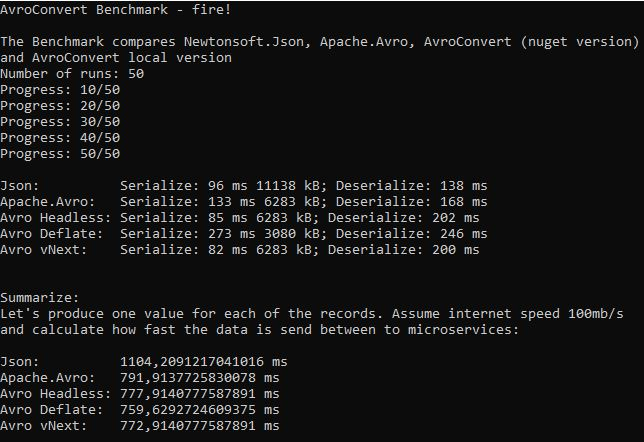
\includegraphics[width=\textwidth]{benchmark}
	\caption{Comparison of result from AvroConvert benchmark}
\end{figure}

All of the implementations of Avro provides quite similar results. The reason, why I didn't choose the official implementation of Avro format in the C\# world (Apache.Avro) is that it doesn't support many key types like decimal, dictionary, list or Guid. 

AvroConvert supports few serialization scenarios:
\begin{enumerate}
	\item Standard serialization - result contains header and data. Like in the given example.
	\item Serialization with additional encoding -  result contains a header (with information about codec type) and encoded data. It decreases the size of the result but increases serialization and deserialization time. Look at the AvroConvert Deflate on the benchmark screen.
	\item Headless serialization  - result contains only data. Assumes, that schema is known upfront. Decreases size of the result, serialization and deserialization time.
\end{enumerate}

To sum up - in the given scenario it doesn't really matter which Avro serialization you will choose. Each of them speed's up the response for about 25-30\%.


\section{How to build Avro API}

And finally - let's code this! The implementation in .NET Core 3.0 is very easy, in fact, we need just 3 classes: 

\begin{itemize}
	\item AvroInputFormatter
	\item AvroOutputFormatter
	\item HttpClient extensions that support Avro format
\end{itemize}

In my implementation serializaiton is done by AvroConvert. Every implementation of Avro serializaiton should be compatible with each other, though.

\subsection{AvroInputFormatter}

\begin{lstlisting}[language={[Sharp]C}, label={Script}]
public class AvroInputFormatter : InputFormatter
{
	public AvroInputFormatter()
	{
		this.SupportedMediaTypes.Clear();
		
		this.SupportedMediaTypes.Add(MediaTypeHeaderValue.Parse("application/avro"));
	}
	
	public override Task<InputFormatterResult> ReadRequestBodyAsync(InputFormatterContext context)
	{
		using (MemoryStream ms = new MemoryStream())
		{
			context.HttpContext.Request.Body.CopyTo(ms);
			var type = context.ModelType;
			
			object result = AvroConvert.Deserialize(ms.ToArray(), type);
			return InputFormatterResult.SuccessAsync(result);
		}
	}
}
\end{lstlisting}

\subsection{AvroOutputFormatter}

\begin{lstlisting}[language={[Sharp]C}, label={Script}]
public class AvroOutputFormatter : OutputFormatter
	{
	public AvroOutputFormatter()
	{
		this.SupportedMediaTypes.Clear();
		
		this.SupportedMediaTypes.Add(MediaTypeHeaderValue.Parse("application/avro"));
	}
	
	public override async Task WriteResponseBodyAsync(OutputFormatterWriteContext context)
	{
		var avroBody = AvroConvert.Serialize(context.Object);
		
		var response = context.HttpContext.Response;
		response.ContentLength = avroBody.Length;
		
		await response.Body.WriteAsync(avroBody);
	}
}
\end{lstlisting}

\subsection{HttpClient extensions}

\begin{lstlisting}[language={[Sharp]C}, label={Script}]
public static class HttpClientExtensions
{
	public static async Task<HttpResponseMessage> PostAsAvro(this HttpClient httpClient, string requestUri, object content)
	{
		var body = new ByteArrayContent(AvroConvert.Serialize(content));
		body.Headers.ContentType = new MediaTypeHeaderValue("application/avro");
		return await httpClient.PostAsync(requestUri, body);
	}
	
	public static async Task<T> GetAsAvro<T>(this HttpClient httpClient, string requestUri)
	{
		var response = await httpClient.GetByteArrayAsync(requestUri);
		T result = AvroConvert.Deserialize<T>(response);
		return result;
	}
}
\end{lstlisting}


\subsection{Modify Startup}
\begin{lstlisting}[language={[Sharp]C}, label={Script}]
services.AddMvc(options =>
{
	options.InputFormatters.Insert(0, new AvroInputFormatter());
	options.OutputFormatters.Insert(0, new AvroOutputFormatter());
});
\end{lstlisting}

And - that's it. You've just speeded up responses of your APIs by at least 30\%. Play with the serialization options, you can achieve even better results. I've gathered the methods used for communication in the separate library: \href{https://github.com/AdrianStrugala/SolTechnology.Avro.Http}{SolTechnology.Avro.Http}.

Thank you for reading the article. I hope you can make good use of the knowledge I just shared. In case of any questions, contact me at strugala.adrian@gmail.com. See you!

\section{Useful links}
\begin{itemize}
	\item http://avro.apache.org/
	\item https://cwiki.apache.org/confluence/display/AVRO/Index
	\item https://github.com/AdrianStrugala/AvroConvert
	\item https://github.com/AdrianStrugala/SolTechnology.Avro.Http
\end{itemize}


\end{document}
